\documentclass[../main.tex]{subfiles}

\usepackage{amsmath}
\usepackage{amssymb}

\usetikzlibrary{calc,intersections,through,backgrounds}

\begin{document}

    \part{Définitions}

        \subpart{Compas}
            \definition{compas}

        \subpart{Cercle}
            \definition{cercle}
            \begin{exemple}\par\noindent
                \begin{minipage}[c]{.45\linewidth}
                    \begin{center}
                        \exported[scale=1,lmargin=30,vmargins=30,active=1]%
                        <<
                            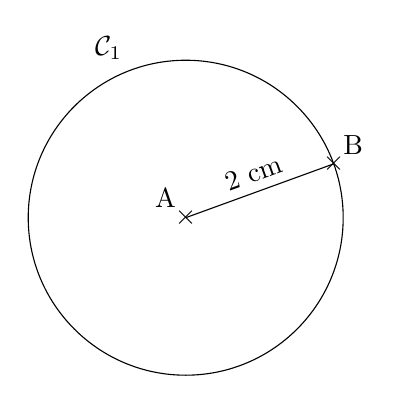
\begin{tikzpicture}[baseline=(A.base)]
                                \coordinate[label=above left:A](A)at(0,0);
                                \coordinate[label=above right:B](B)at(20:2);
                                \draw(A)circle(2);
                                \draw(A)--(B)node[pos=0.5,sloped,above]{2 cm};
                                \node at(A){$\times$};
                                \node at(B){$\times$};
                                \node[above left]at(110:2){$\mathcal{C}_1$};
                            \end{tikzpicture}
                        >>
                    \end{center}
                \end{minipage}\hspace{.08\linewidth}
                \begin{minipage}[c]{.45\linewidth}
                    Le cercle $\mathcal{C}_1$ est :
                    \begin{itemize}
                        \item l'ensemble des points qui se situent
                        à \textsf{2 cm} du point \textsf{A}.
                        \item le cercle de centre \textsf{A} et de
                        rayon \textsf{2 cm}.
                        \item le cercle de centre \textsf{A} passant par \textsf{B}.
                    \end{itemize}
                \end{minipage}
            \end{exemple}
            \begin{remarque}
                Le mot \guillemets{rayon} désigne aussi bien la distance du centre
                à un point du cercle que le segment reliant ces deux points:
                \begin{itemize}
                    \item \relax[\textsf{AB}] est un rayon du cercle.
                    \item Le rayon du cercle vaut 2 cm.
                \end{itemize}
            \end{remarque}

    \part{Applications}

        \subpart{Constructions de cercle}
        \begin{exemple}
            \begin{enumerate}[i), font=\bfseries]
                \item Placer un point \textsf{O}.
                \item Tracer le cercle de centre \textsf{O} de rayon 4,5 cm.
            \end{enumerate}
            Le diamètre du cercle vaut 9 cm.
        \end{exemple}
        \begin{exemple}
            \begin{enumerate}[i), font=\bfseries]
                \item Placer un point \textsf{C}.
                \item Tracer le cercle de centre \textsf{C} de diamètre 7 cm.
            \end{enumerate}
            Le rayon du cercle vaut 3,5 cm.
        \end{exemple}
        \begin{exemple}
            \begin{enumerate}[i), font=\bfseries]
                \item Placer un point \textsf{F}.
                \item Placer un point \textsf{E} dinstinct du point \textsf{F}.
                \item Tracer le cercle de centre \textsf{E} passant par \textsf{F}.
            \end{enumerate}
        \end{exemple}

        \subpart{Constructions de triangles}
        \begin{exemple}
            Tracer un triangle \textsf{CBA} tel que:
            \begin{itemize}
                \item$\textsf{AC}=5$ cm
                \item$\textsf{AB}=4$ cm
                \item$\textsf{BC}=3$ cm
            \end{itemize}
            Le programme de tracé détaillé est le suivant:
            \begin{enumerate}[i), font=\bfseries]
                \item Tracer [\textsf{AC}] tel que $\textsf{AC}=5$ cm.
                \item Tracer le cercle de centre \textsf{A} et de rayon 4 cm.
                \item Tracer le cercle de centre \textsf{C} et de rayon 3 cm.
                \item Placer le point B sur une des intersections de deux cercles.
                \item Tracer [\textsf{AB}] et [\textsf{BC}].
            \end{enumerate}
        \end{exemple}
        \begin{exemple}
            Tracer un triangle \textsf{IJK} tel que:
            \begin{itemize}
                \item$\textsf{JK}=6$ cm
                \item$\widehat{\sf IJK}=50$\^\circ$$
                \item$\textsf{IK}=4,5$ cm
            \end{itemize}
            Le programme de tracé détaillé est le suivant:
            \begin{enumerate}[i), font=\bfseries]
                \item Tracer [\textsf{JK}] tel que $\textsf{JK}=6$ cm.
                \item Placer un point E tel que $\widehat{\sf EJK}=50$\^\circ$$.
                \item Tracer le cercle $\mathcal{C}_0$ de centre \textsf{K} et de rayon 4,5 cm.
                \item Placer le point I à l'intersection de [\textsf{JE}) et du cercle
                $\mathcal{C}_0$.
            \end{enumerate}
        \end{exemple}
\end{document}